%%
\documentclass[format=draft,language=chinese,category=SDN]{hustreport}
\hypersetup{
    colorlinks=true,
    linkcolor=blue,
    filecolor=magenta,
    urlcolor=cyan,
}

\title{初赛文档}
\author{\kai{林家军}~~\kai{李英儒}~~\kai{胡云锐}}
\major{计算机科学与技术}
\department{计算机科学与技术学院}
\advisor{\kai{周世伟}}

\abstract{
    这是来自华中科技大学UniqueSDNStudio队伍的初赛文档,于\LaTeX{}编辑而成。

}
\keywords{软件定义网络, SDN, \LaTeX{}, 华中科技大学}


\begin{document}
\nocite{*}

\frontmatter
\maketitle
\makeabstract
\tableofcontents
\listoffigures
\listoftables
\mainmatter

\chapter{基础环境}\label{chapter:BaiscEnv}
SDN 的基础环境由 SDN 控制器(Controller)和支持 SDN 的交换机构成
的网络组成,我们在本次比赛中使用 Ryu 作为 SDN 控制器,使用 Mininet 构建
虚拟试验网络。
\section{Ryu}
Ryu is a component-based software defined networking framework.

Ryu是一个基于组件的软件定义网络框架。

Ryu provides software components with well defined API that make it easy for developers to create new network management and control applications. Ryu supports various protocols for managing network devices, such as OpenFlow, Netconf, OF-config, etc. About OpenFlow, Ryu supports fully 1.0, 1.2, 1.3, 1.4 and Nicira Extensions.

Ryu提供了具有良好设计的API结构的软件组件,使得开发者能够更加方便简单地创建新的网络管理控制应用。Ryu支持许多管理网络设备的协议,例如OpenFlow, Netconf, OF-config等。关于Openflow,Ryu支持全部1.0, 1.2, 1.3, 1.4和Nicira扩展。

All of the code is freely available under the Apache 2.0 license. Ryu is fully written in Python.

所有Ryu代码能够在Apache 2.0 许可下自由地获取。 Ryu全部由Python写成。

\section{Mininet}
Mininet 是由一些虚拟的终端节点(end-hosts)、交换机、路由器连接而成的一个网络仿真器,它采用轻量级的虚拟化技术使得系统可以和真实网络相媲美。它可以很方便的创建一个支持 SDN 的网络,有了这个网络,就可以灵活的为网络添加新的功能并进行相关测试。

\chapter{参赛情况}\label{chapter:Situation}


\section{竞赛组织及参与情况}
本次竞赛的组织活动由校教务处发起,在全校范围内自主报名参加。联创团队组织三名大二学生参赛,并安排一位研究生作为领队。在参赛过程中,每周每人大约工作时间 40 小时且每周六进行一次讨论总结上周情况并对下周进行科学严谨的安排,为保证作品按时完成我们建立了邮件列表与在线讨论平台,同一管理协调。
\section{参赛队伍构成}
\subsection{联创团队}
联创团队$(Unique Studio)$于 2000 年 6 月创建于华中科技大学,是 $Teamwork$ 和
 $Creation$ 为团队核心的学生团队。团队名称来源于“联众人之智”必能“创辉煌之事”的信念
。联创团队建立了一个自主的精英学生平台,在这个平台上学生自我管理,通过这个平台激发无限的潜力和创意。
自成立到现在,联创团队已参加微软创新杯 11 次并 8 次进入全球总决赛拿下包括全球冠军等优秀成绩。
除此之外,联创团队也多次参加各种大小型比赛并取得了骄人的成绩,并与$MICROSOFT$\texttrademark、$CSDN$\texttrademark 等公司保持着非常好的合作关系,同时加入微软中国组织的创新联盟。
联创团队多年的发展积累了独特的文化和运作机制,同时跟踪技术发展的最前沿,这使得联创团队在华科乃至全国高校中独树一帜。
\subsection{领队}
\kai{周世伟}

\textbf{华中科技大学\textregistered} 2010级本科生,2014 级研究生,现就读于光电与电子信息学院光电信息工程专业。华中科技大学联创团队 IT 组和嵌入式组成员。曾 2 次获得国家奖学金。参与 微软创新杯$Imagine~Cup\texttrademark$ $IT~Challenge\textregistered$ 比赛,并进入中国区总决赛。曾获得
中国区第一届 $RDMA\textregistered$ 比赛一等奖。目前已获得华中科技大学保研资格。
\href{http://zhoushiwei1992.blog.163.com}{周世伟个人博客。}
\subsection{参赛队员}
\kai{林家军}

\textbf{华中科技大学}\textregistered 2013 级本科生,现就读于计算机科学与技术学院计算机科学与技术专业。华中科技大学联创团队 IT 组成员。

\kai{李英儒}

\textbf{华中科技大学}\textregistered 2013 级本科生,现就读于计算机科学与技术学院计算机科学与技术专业。华中科技大学联创团队 IT 组成员。

\kai{胡云锐}

\textbf{华中科技大学}\textregistered 2013 级本科生,现就读于计算机科学与技术专业。
华中科技大学联创团队 IT 组成员,主要进行网络通讯、大数据方面的研究。

\chapter{初赛题目}\label{chapter:Questions}


\section{第一题:基础题}\label{sec:Q1}
\subsection{第1小题:简单网络}\label{sec:Q1_1}

\begin{figure}[!h]
\centering
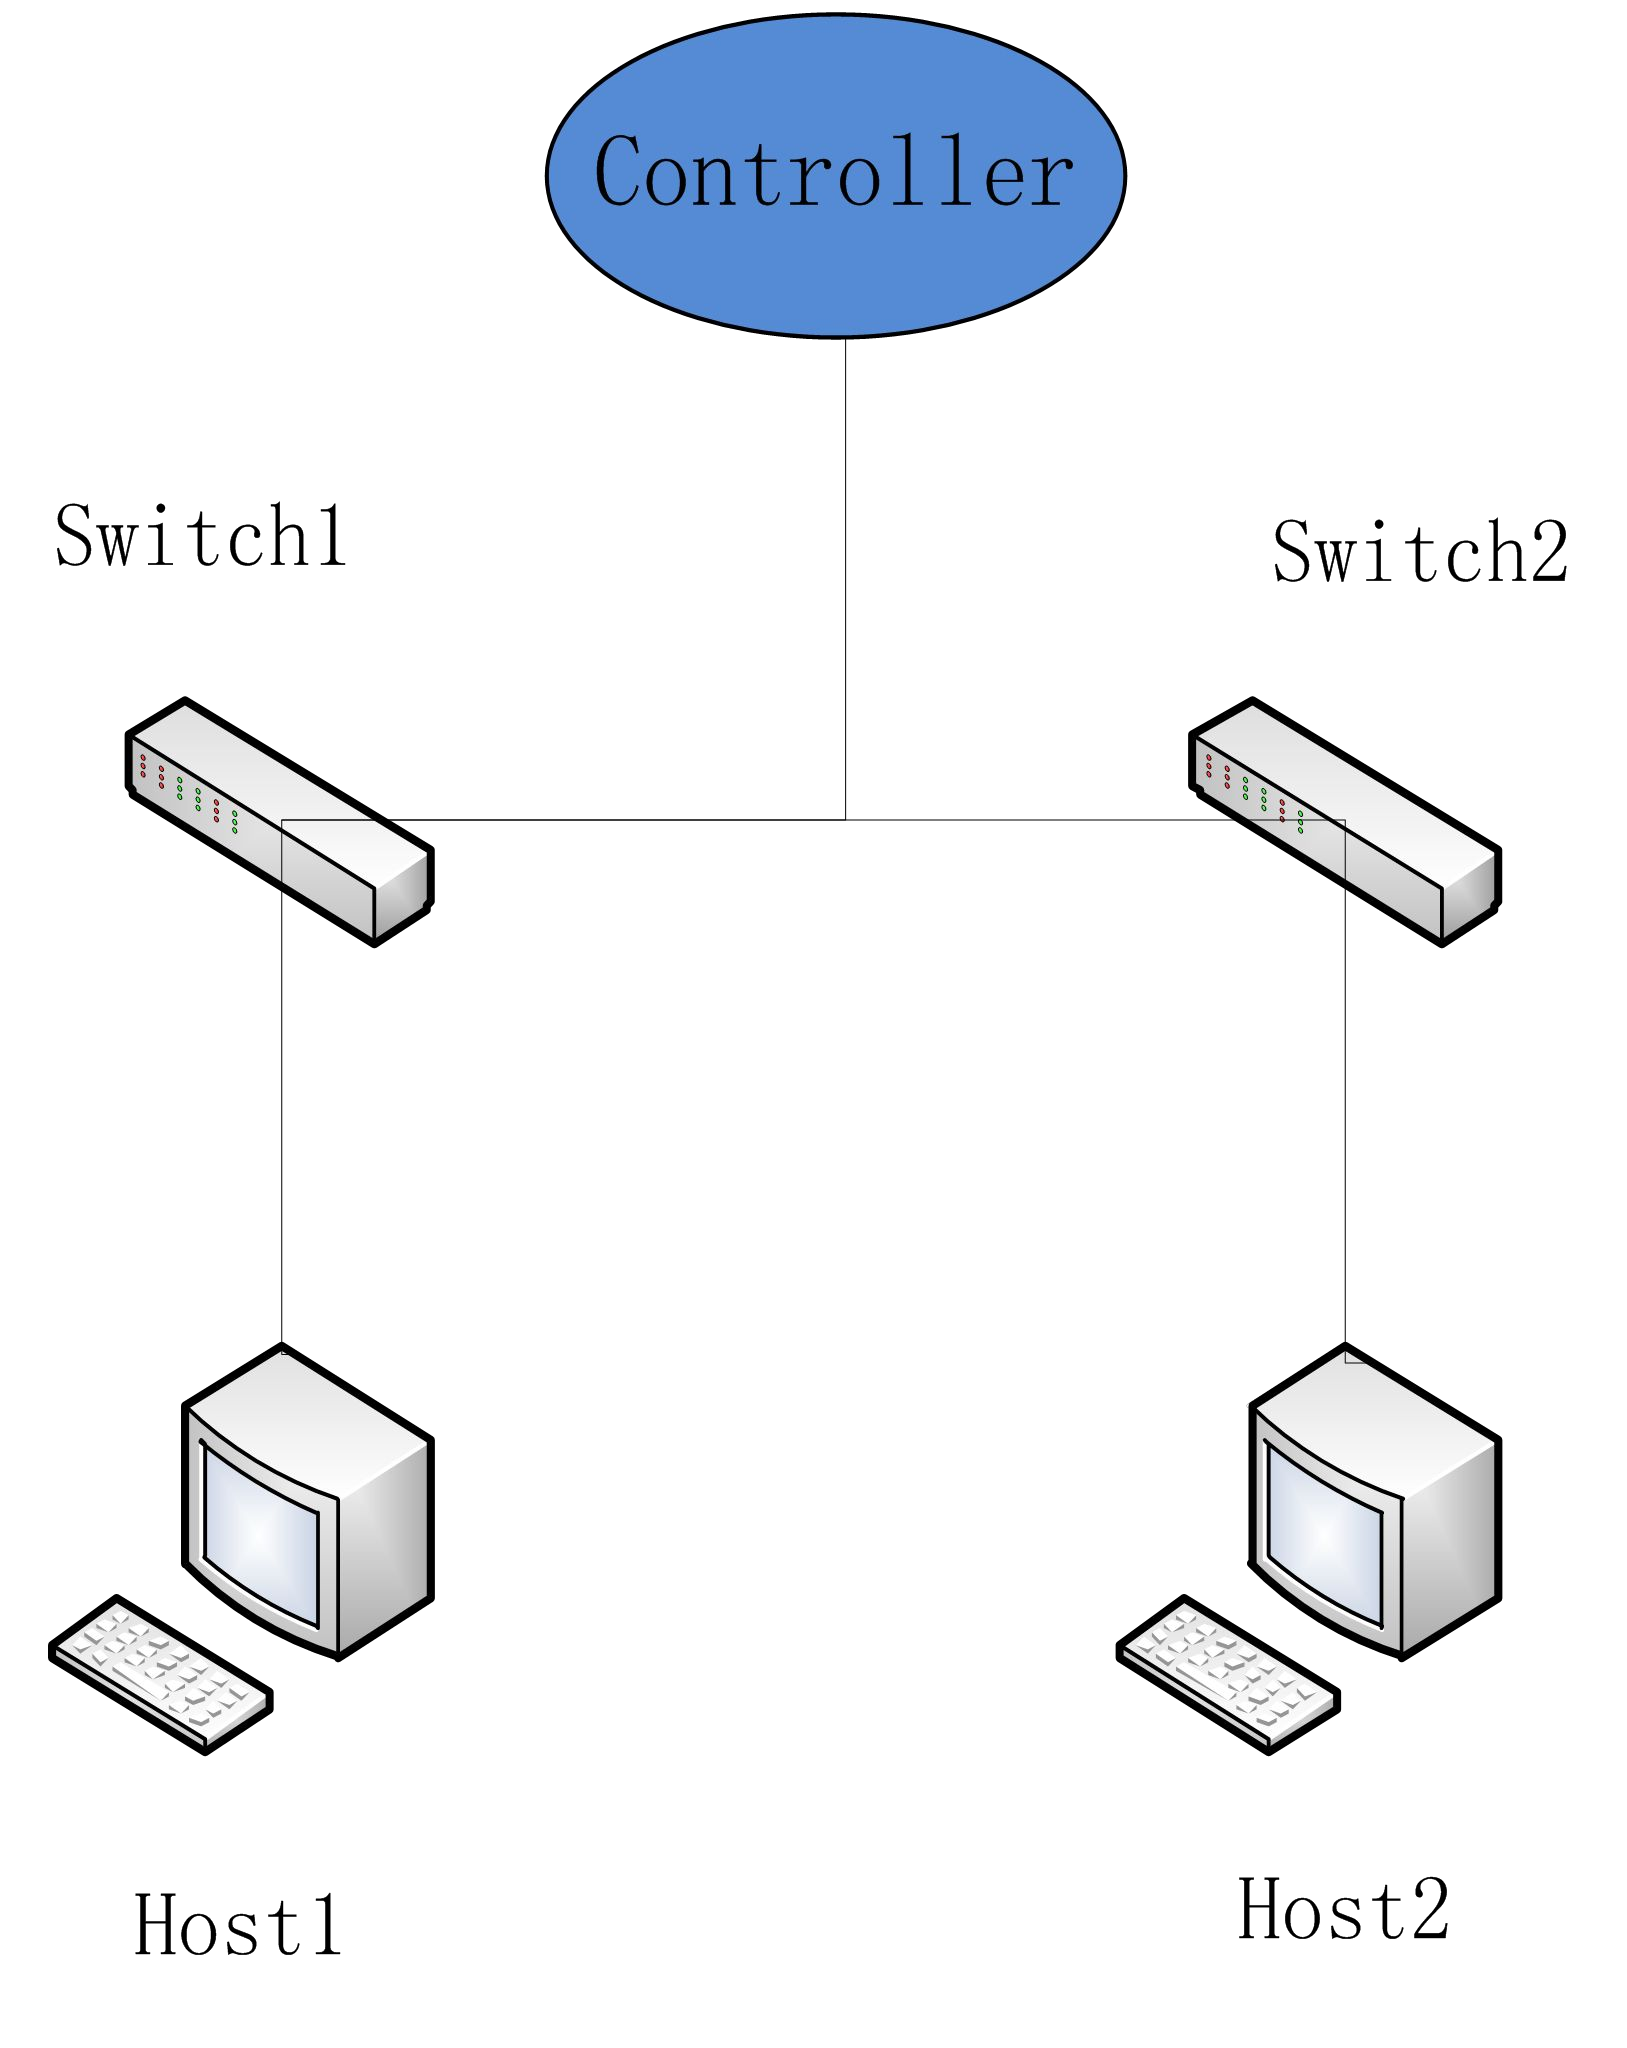
\includegraphics[width=.618\textwidth]{fig/1_1-0.png}
\caption{第一题第1小题:简单网络}\label{fig:Q1_1-0}
\end{figure}

网络环境要求:

要求搭建的网络环境如图 1 所示(controller 表示控制器, switch 表示交换机, host表示主机)。控制器可以自主选择,例如各种开源的控制器(Floodlight、Ryu、
Nox、Beacon、Trema、OpenDaylight 等)。拓扑中各网络部件既可以是仿真环境实现(例如 mininet, OpenvSwtich 等),有条件的队伍也可以通过物理设备实现,
各种方案不影响评分。试题中每道题都遵循这些要求,不再说明。

操作要求:

1.先使 Host1 可以 ping 通 Host2,Host2 也可以 ping 通 Host1。

2.然后对流表进行操作,使 Host1 不能 ping 通 Host2, Host2 也不能 ping 通 Host1。

实验报告要求:

1.详细描述网络环境的搭建思路,列举选择的具体设备或者仿真软件,并说明其在网络环境中的作用。

2.给出实现操作要求的具体步骤,以说明文字和截图展示。

\subsection{第2小题:访问限制}\label{sec:Q1_2}

\begin{figure}[!h]
\centering
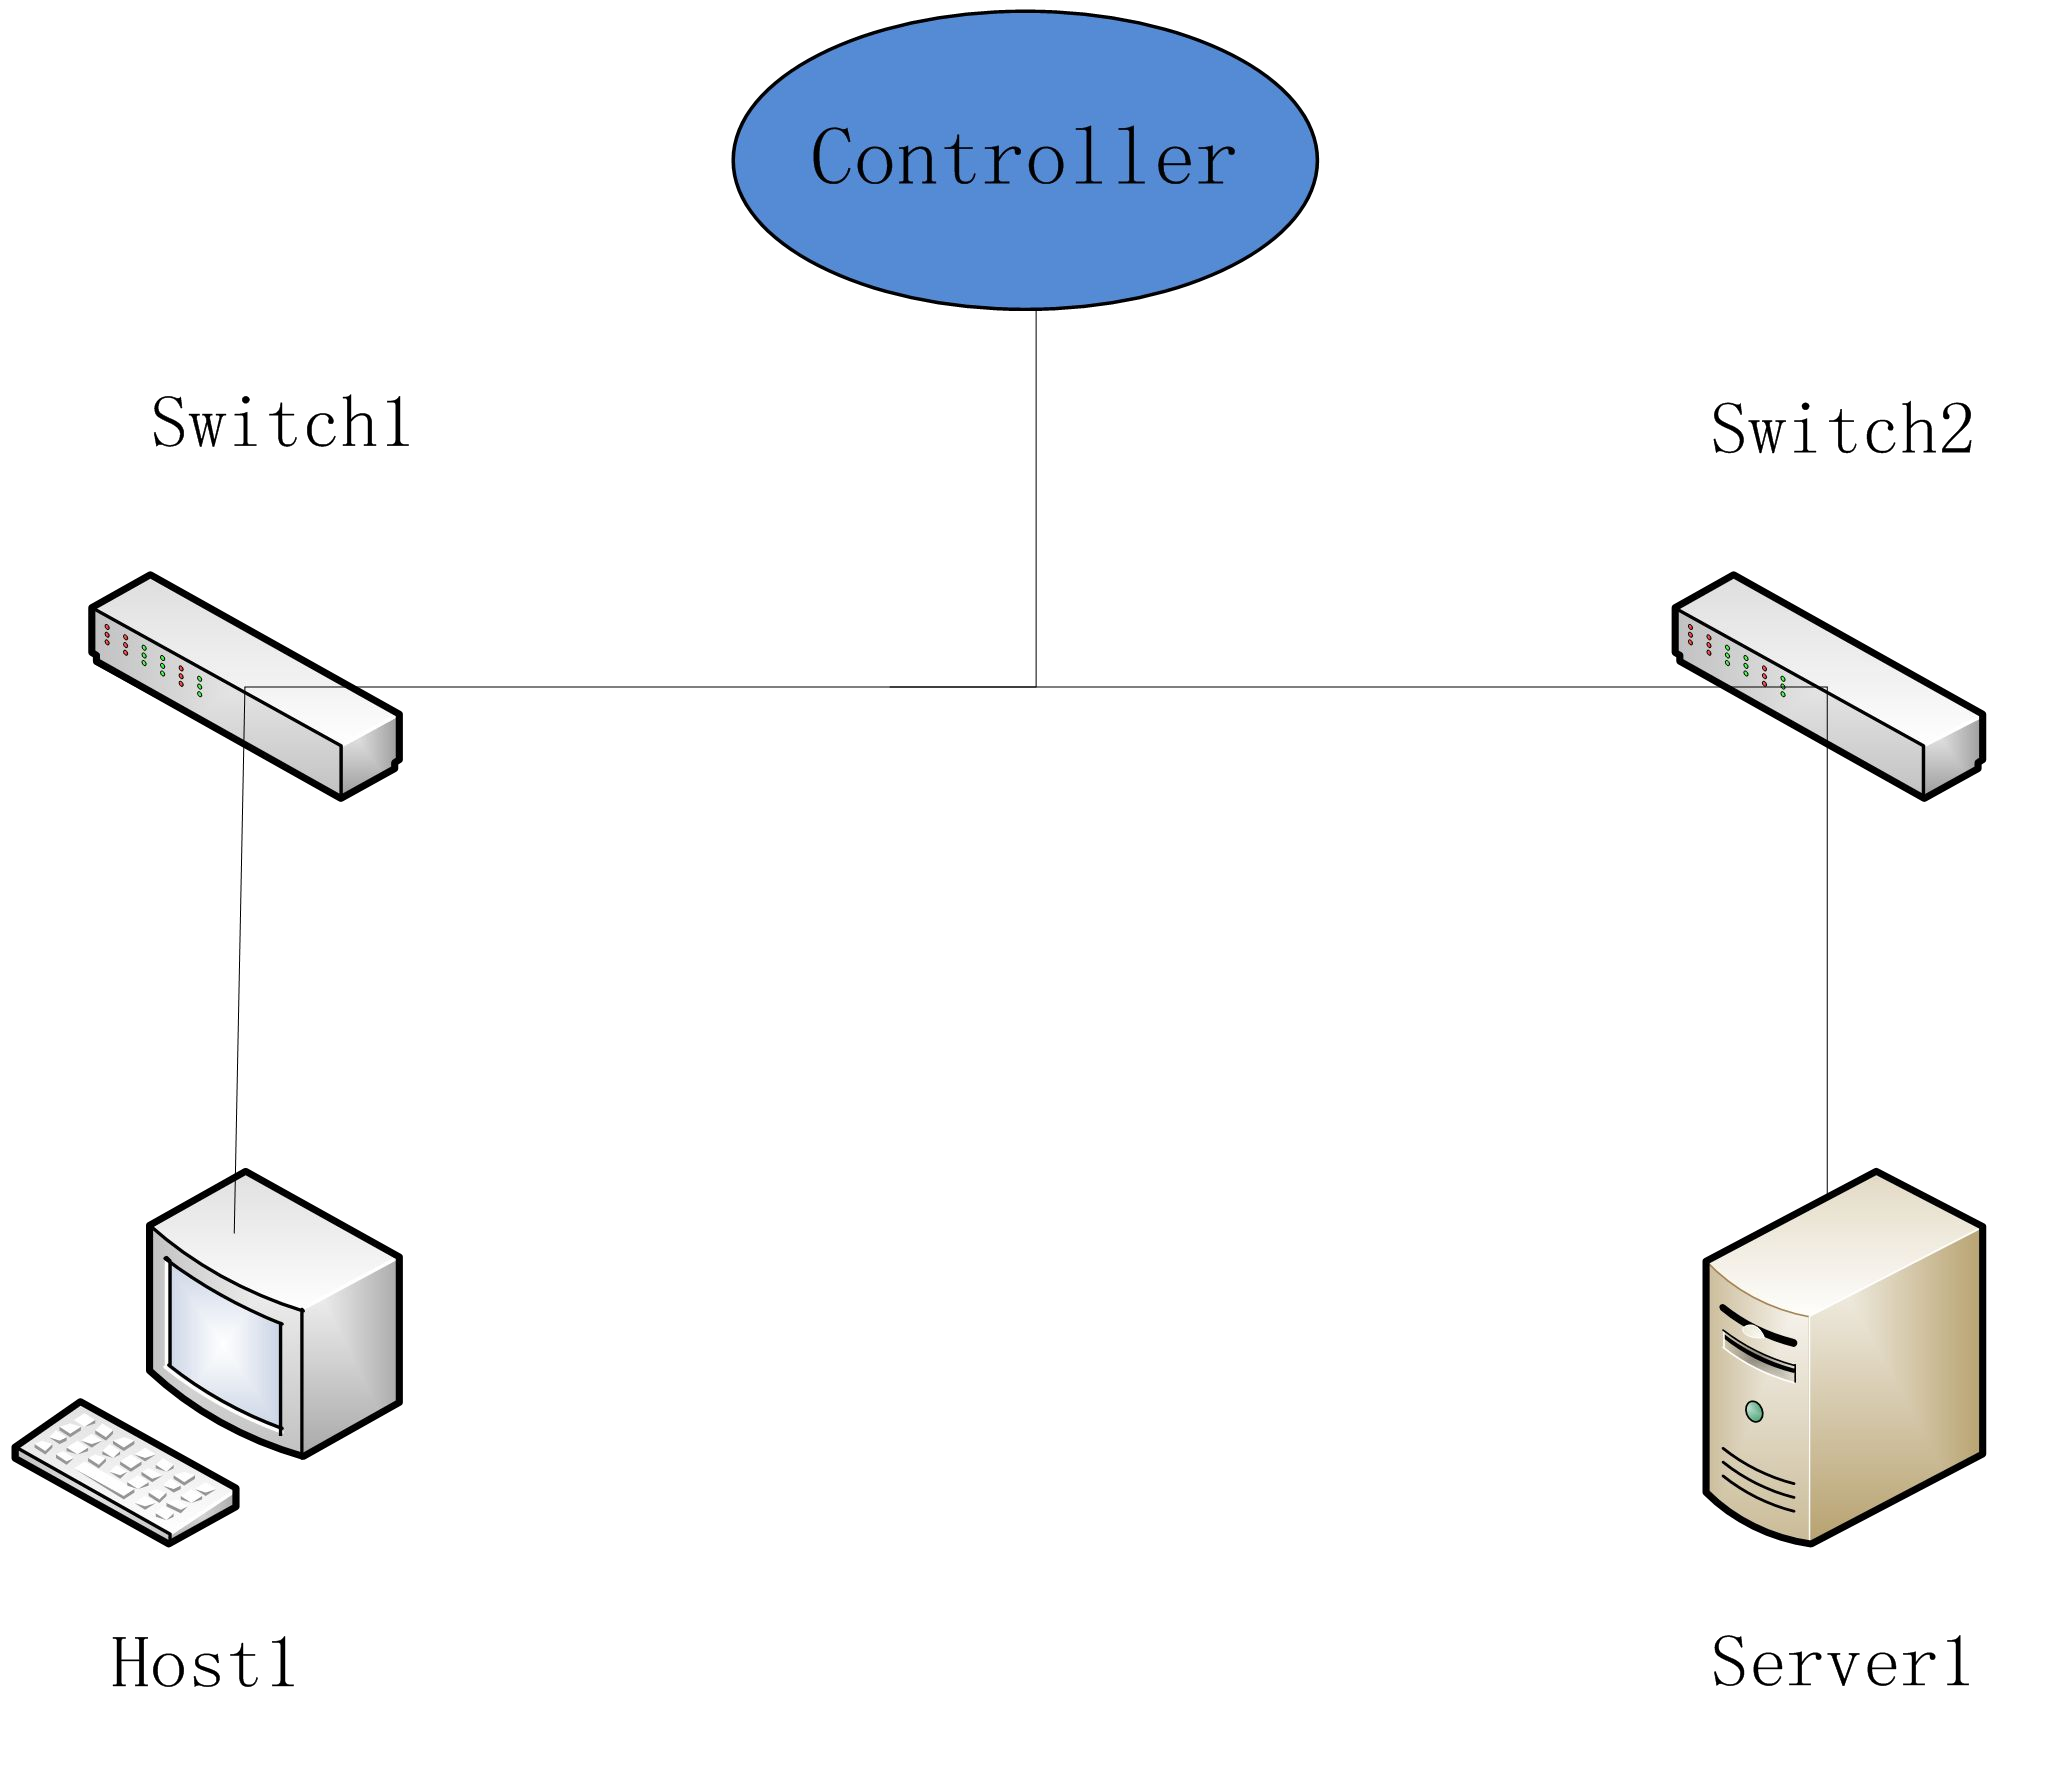
\includegraphics[width=.618\textwidth]{fig/1_2-0.png}
\caption{第一题第1小题:访问限制}\label{fig:Q1_2-0}
\end{figure}

网络环境要求:

设有一台 PC 机(Host1),一台 Web 服务器(Server1)提供简单的静态网页访问服务,如图 2 所示。(PC 机、Web 服务器、交换机、控制器可以选择物理设备或者虚拟设备实现)

操作要求:
1.先使得 PC 机访问服务器成功(即看到服务器的网页)。

2.限制该 PC 机一定时间(比如一分钟)内再次访问服务器。限制时间过后,PC机可以成功访问服务器。

实验报告要求:

1.简要描述网络拓扑,给出拓扑图,说明用什么设备实现该拓扑。

2.给出操作步骤和实验数据,验证是否达到要求。

\section{第二题:提高题}\label{sec:Q2}
\subsection{第1小题:代理访问}\label{sec:Q2_1}

\begin{figure}[!h]
\centering
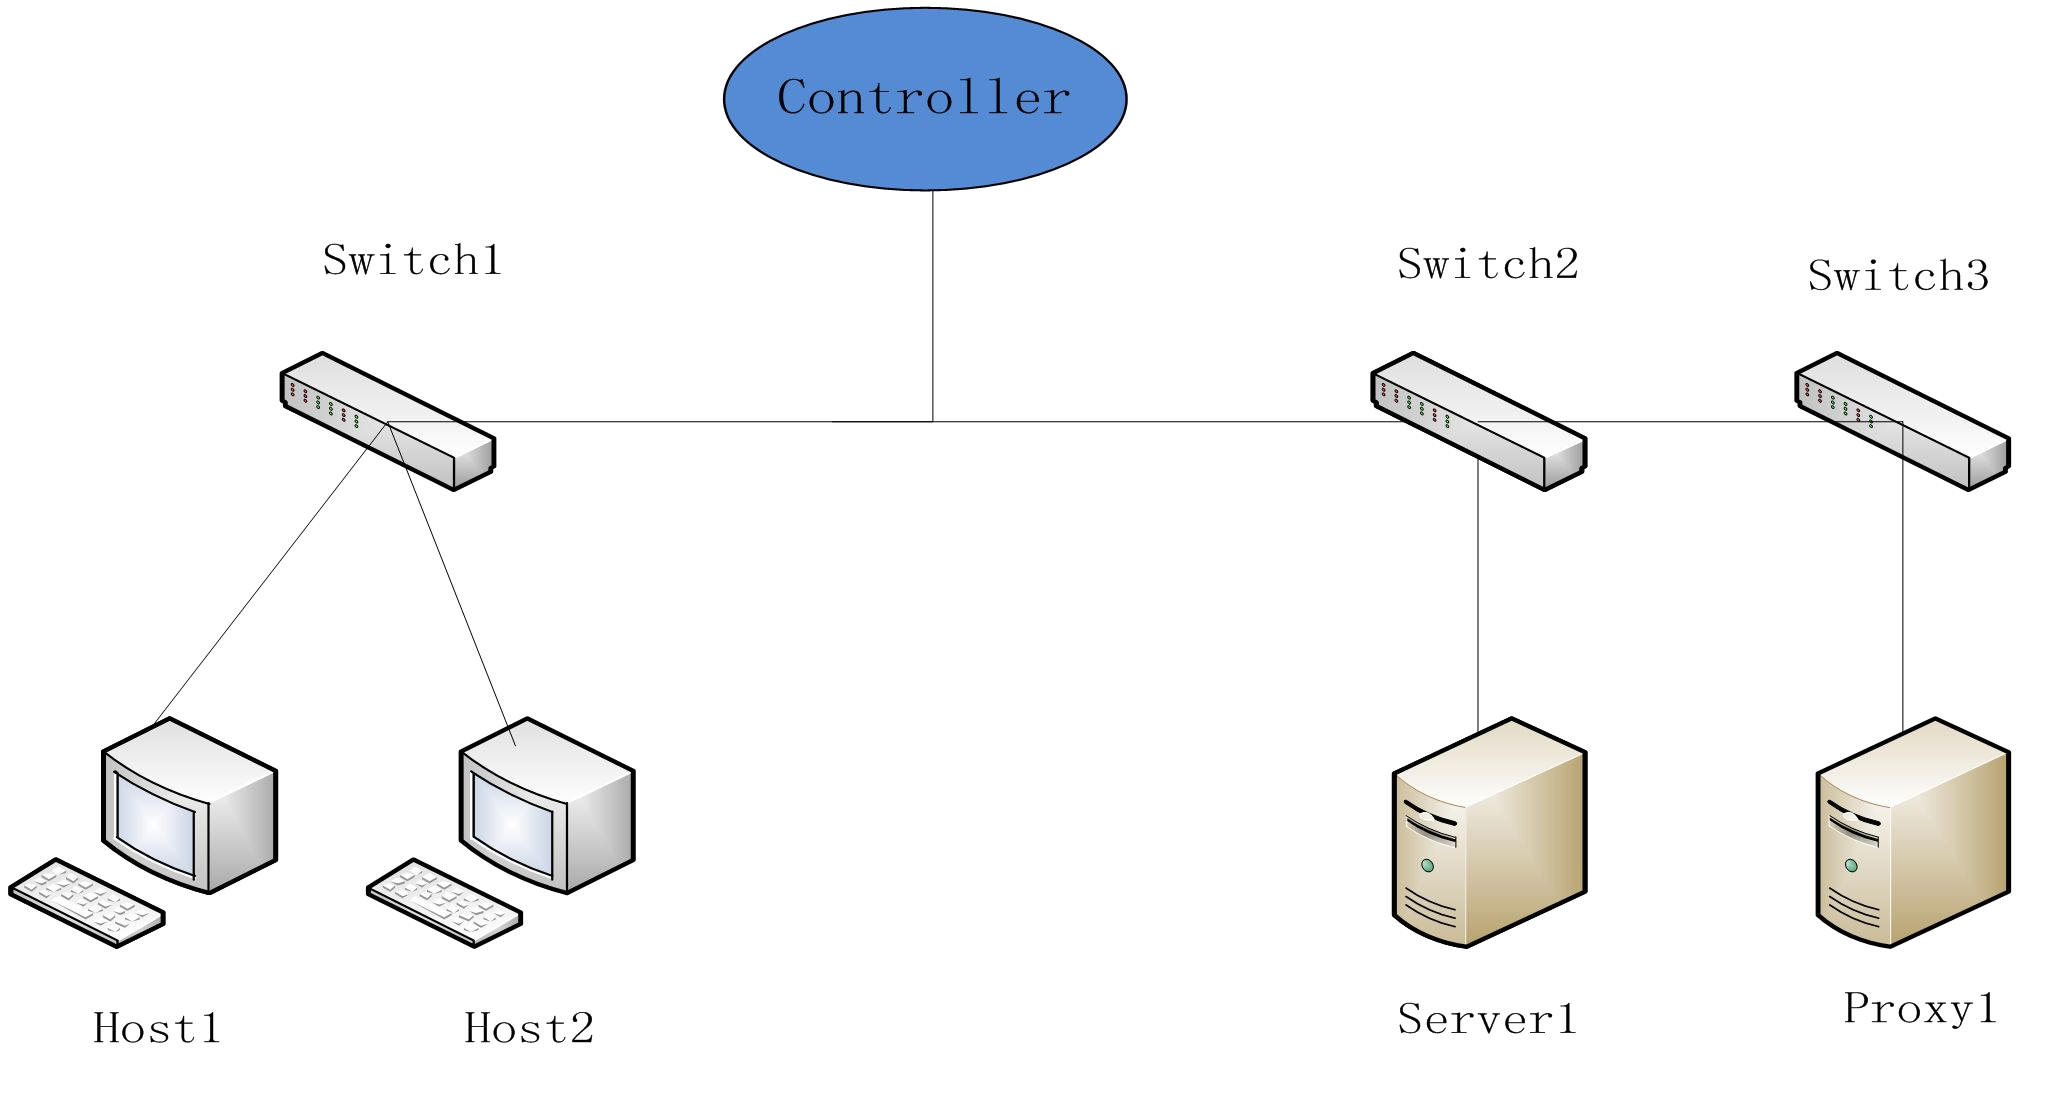
\includegraphics[width=.618\textwidth]{fig/2_1-0.png}
\caption{第二题第1小题:代理访问}\label{fig:Q2_1-0}
\end{figure}

网络环境要求:

设有两台 PC 机(Host1,Host2),一台 Web 服务器(Server1)提供简单的静态网页访问服务,一台代理服务器(Proxy1)和 Web 服务器提供同样的服务,两
台服务器所显示的网页大致相同,但要有显著差别,可以是不同的网页内容或者不同颜色,能够区分彼此即可,如图 3 所示。(PC 机、Web 服务器、代理服务器、交换机、控制器可以选择物理设备或者虚拟设备实现)

操作要求:

1.Web 服务器是 Host1 和 Host2 都可以访问的,而代理服务器是只有代理用户才可以使用。

2 可以设置 Host1 或 Host2 为代理用户,可以直接从代理服务器访问到网页。

实验报告要求:

1.简要描述网络拓扑,给出拓扑图,说明用什么设备实现该拓扑。

2.给出操作步骤。

3.给出实验数据,验证是否达到要求。

\subsection{第2小题:流表管理}\label{sec:Q2_2}

\begin{figure}[!h]
\centering
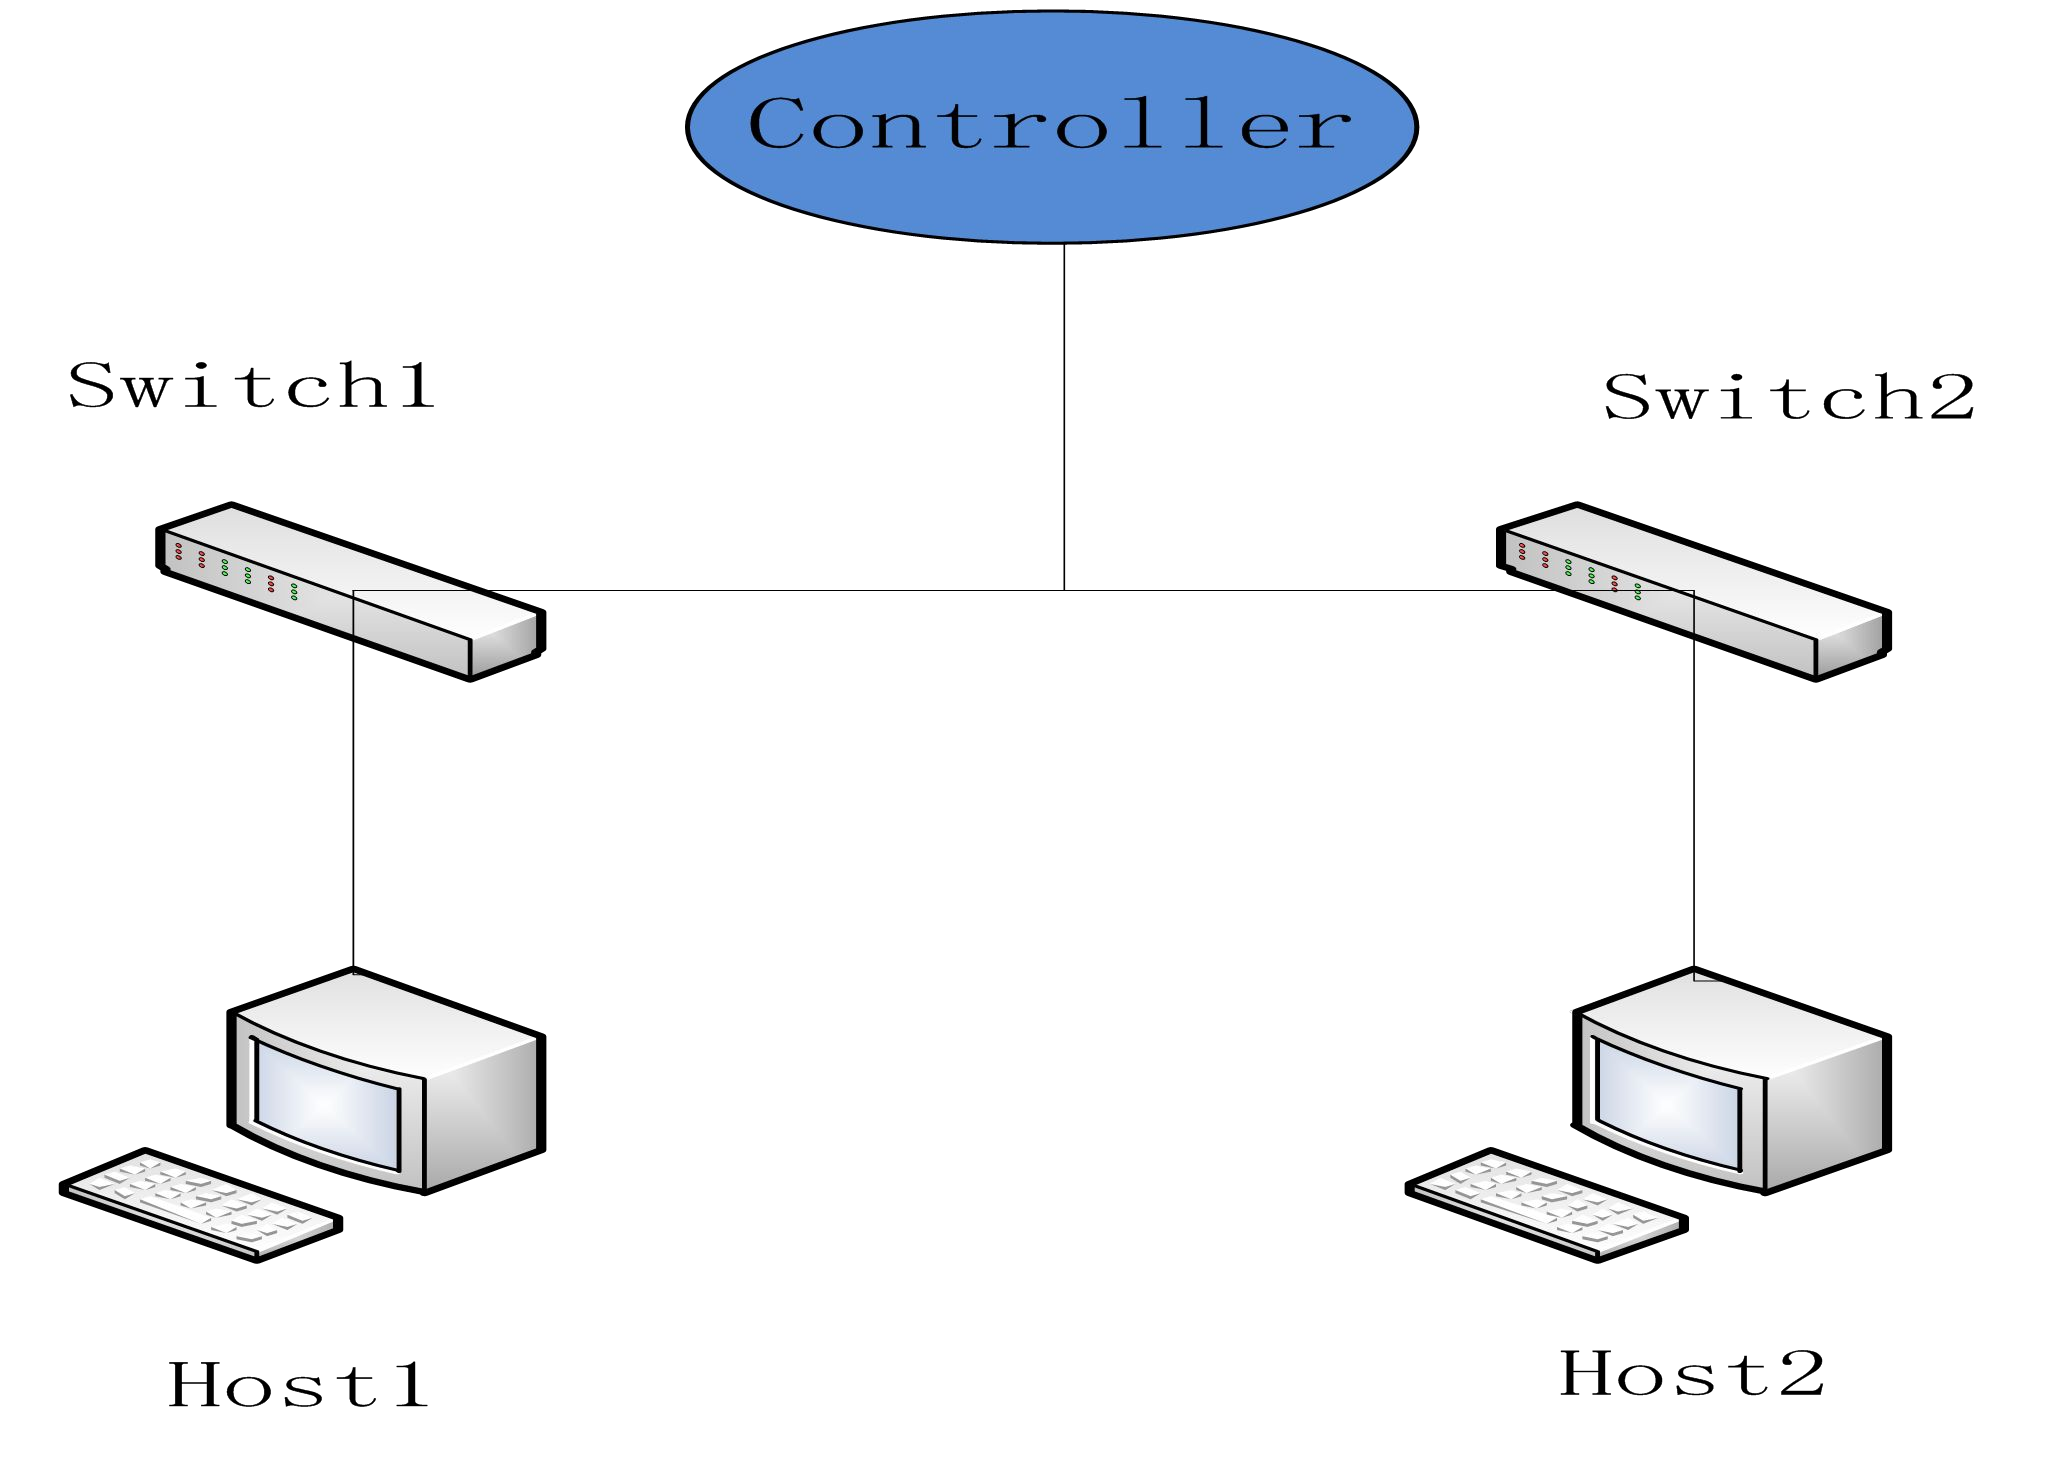
\includegraphics[width=.618\textwidth]{fig/2_2-0.png}
\caption{第二题第2小题:流表管理}\label{fig:Q2_2-0}
\end{figure}

网络环境要求:

设有若干台 PC 机(Host1,Host2),若干台交换机(Switch1,Switch2),如图 4所示(作为示例拓扑,实际拓扑可自由选择)。(PC 机、交换机、控制器可以选择物理设备或者虚拟设备实现)

操作要求:

利用控制器提供的 API(例如 REST API),开发一个网络及流表管理工具(客户端,网页端均可)。管理工具可以显示网络拓扑结构,查看流表,增加流表,删除流表。
实验报告要求:

1.简要描述网络拓扑,给出拓扑图,说明用什么设备实现该拓扑。

2.给出开发管理工具的过程,以及代码。

3.给出实验数据,验证是否达到要求。

\section{第三题:设计题}\label{sec:Q3}

\subsubsection{第三层}\label{sec:3}
测试测试测试测试测试测试测试测试测试测试测试测试。
\footnote{\label{footnote:1}脚注}

\section{字体}

普通\textbf{粗体}\emph{斜体}

\hei{黑体}\kai{楷体}\fangsong{仿宋}

\section{公式}

单个公式,公式引用:\autoref{eq:1}。
\begin{equation}
 c^2 = a^2 + b^2 \label{eq:1}
\end{equation}

多个公式,公式引用:\autoref{eq:2},\autoref{eq:3}。

\begin{subequations}
\begin{equation}
  F = ma \label{eq:2}
\end{equation}
\begin{equation}
  E = mc^2 \label{eq:3}
\end{equation}
\end{subequations}

\section{罗列环境}

\begin{enumerate}
    \item 第一层\label{item:1}
    \item 第一层
    \begin{enumerate}
        \item 第二层\label{item:2}
        \item 第二层
        \begin{enumerate}
            \item 第三层\label{item:3}
            \item 第三层
        \end{enumerate}
    \end{enumerate}
\end{enumerate}

\begin{description}
    \item[解释环境]  解释内容
\end{description}

\chapter{其他格式测试}

\section{代码环境}

\begin{lstlisting}[language=python]
import os

def main():
    '''
    doc here
    '''
    print 'hello, world' # Abc
    print 'hello, 中文' # 中文
\end{lstlisting}

\section{定律证明环境}

\begin{definition}\label{def:1}
这是一个定义。
\end{definition}
\begin{proposition}\label{proposition:1}
这是一个命题。
\end{proposition}
\begin{axiom}\label{axiom:1}
这是一个公理。
\end{axiom}
\begin{lemma}\label{lemma:1}
这是一个引理。
\end{lemma}
\begin{theorem}\label{theorem:1}
这是一个定理。
\end{theorem}
\begin{proof}\label{proof:1}
这是一个证明。
\end{proof}

\section{算法环境}

\begin{algorithm}[H]
\SetAlgoLined
\KwData{this text}
\KwResult{how to write algorithm with \LaTeX2e }
initialization\;\label{alg_line:1}
\While{not at end of this document}{
read current\;
\eIf{understand}{
go to next section\;
current section becomes this one\;
}{
go back to the beginning of current section\;
}
}
\caption{How to write algorithms}\label{alg:1}
\end{algorithm}

\section{表格}
表格见\autoref{tab:1}。

\begin{table}[!h]
\centering
\caption{一个表格}\label{tab:1}
\begin{tabular}{|c|c|}
\hline
a & b \\
\hline
c & d \\
\hline
\end{tabular}
\end{table}
\section{图片}
图片见\autoref{fig:1}。图片格式支持eps,png,pdf等。多个图片见\autoref{fig:2},分开引用:\autoref{fig:2-1},\autoref{fig:2-2}。

\begin{figure}[!h]
\centering
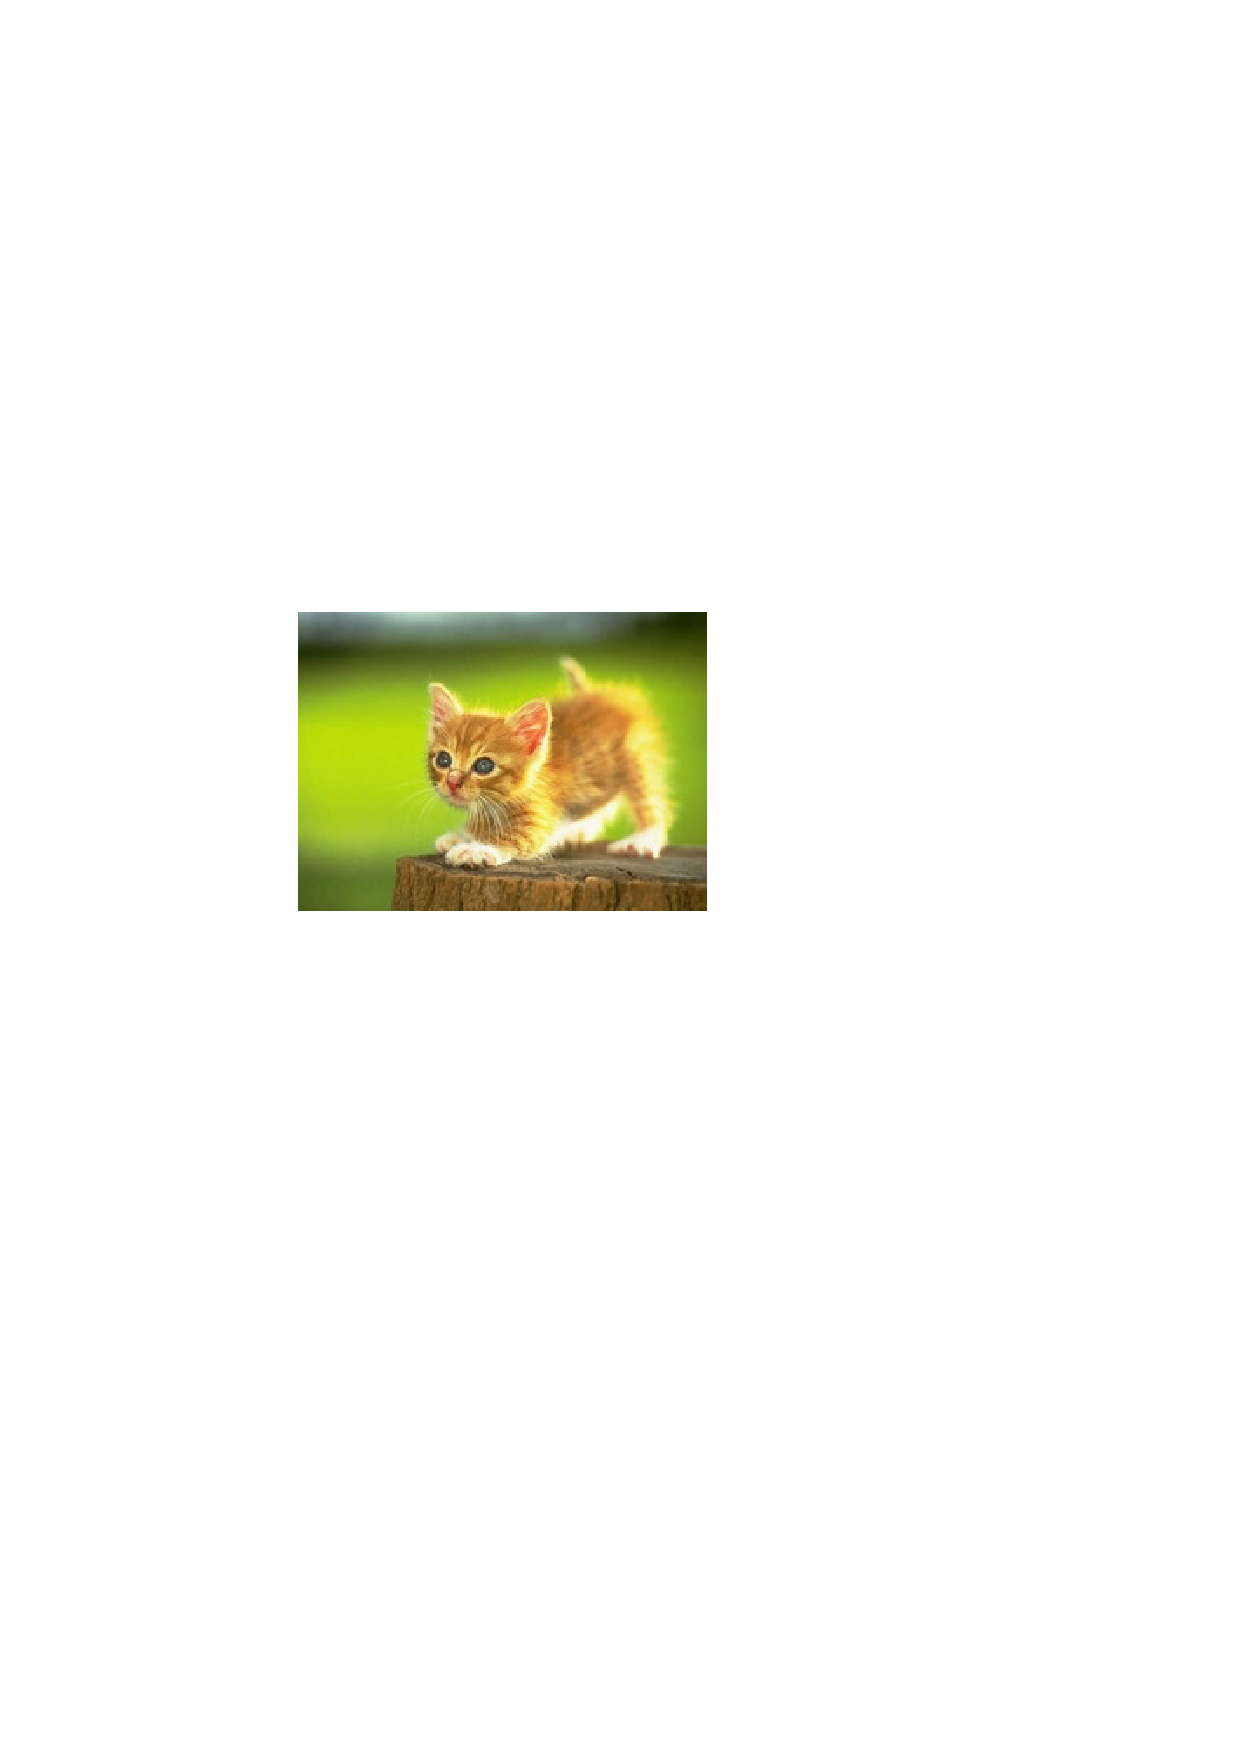
\includegraphics[width=.4\textwidth]{fig/fig-example.pdf}
\caption{一个图片}\label{fig:1}
\end{figure}

\begin{figure}[!h]
\centering
  \begin{subfigure}[b]{0.3\textwidth}
  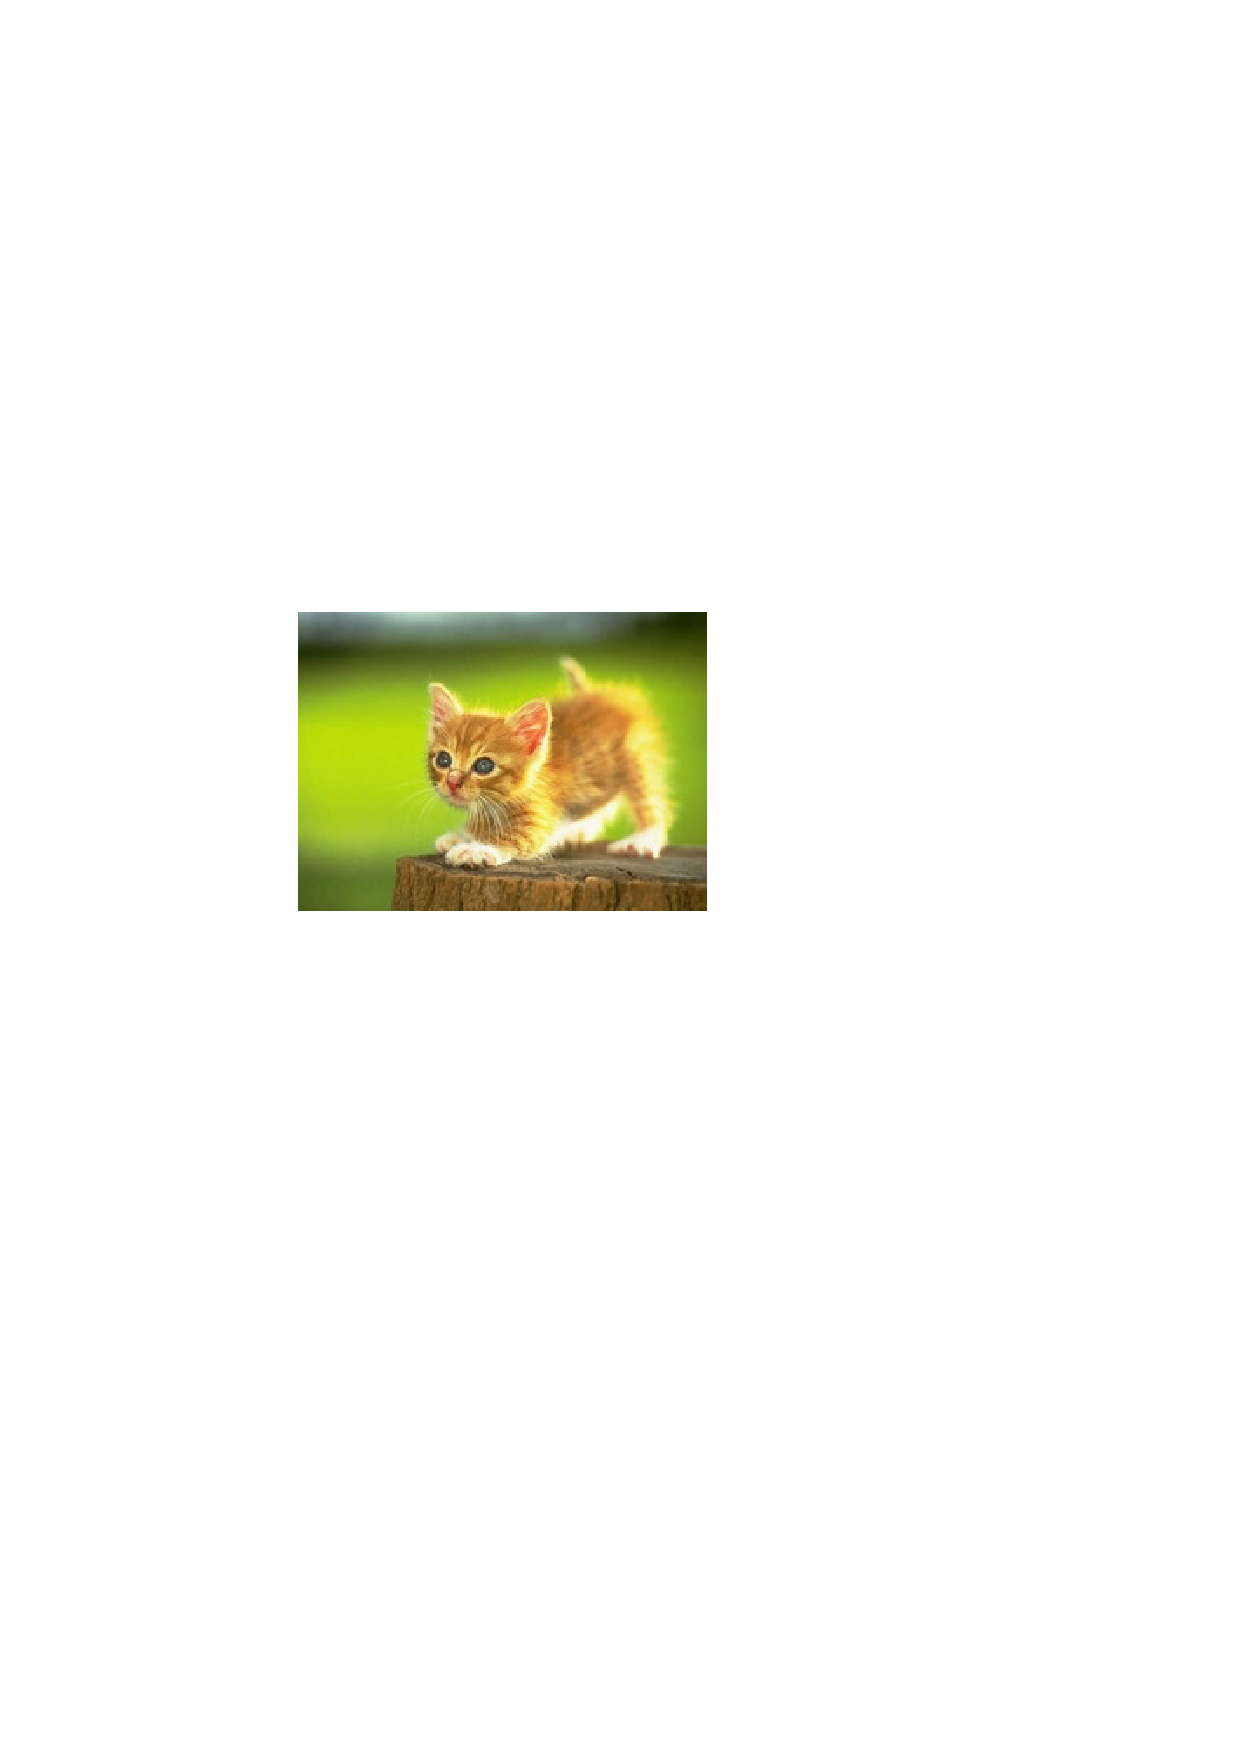
\includegraphics[width=\textwidth]{fig/fig-example.pdf}
  \caption{图片1}\label{fig:2-1}
  \end{subfigure}
  ~
  \begin{subfigure}[b]{0.3\textwidth}
  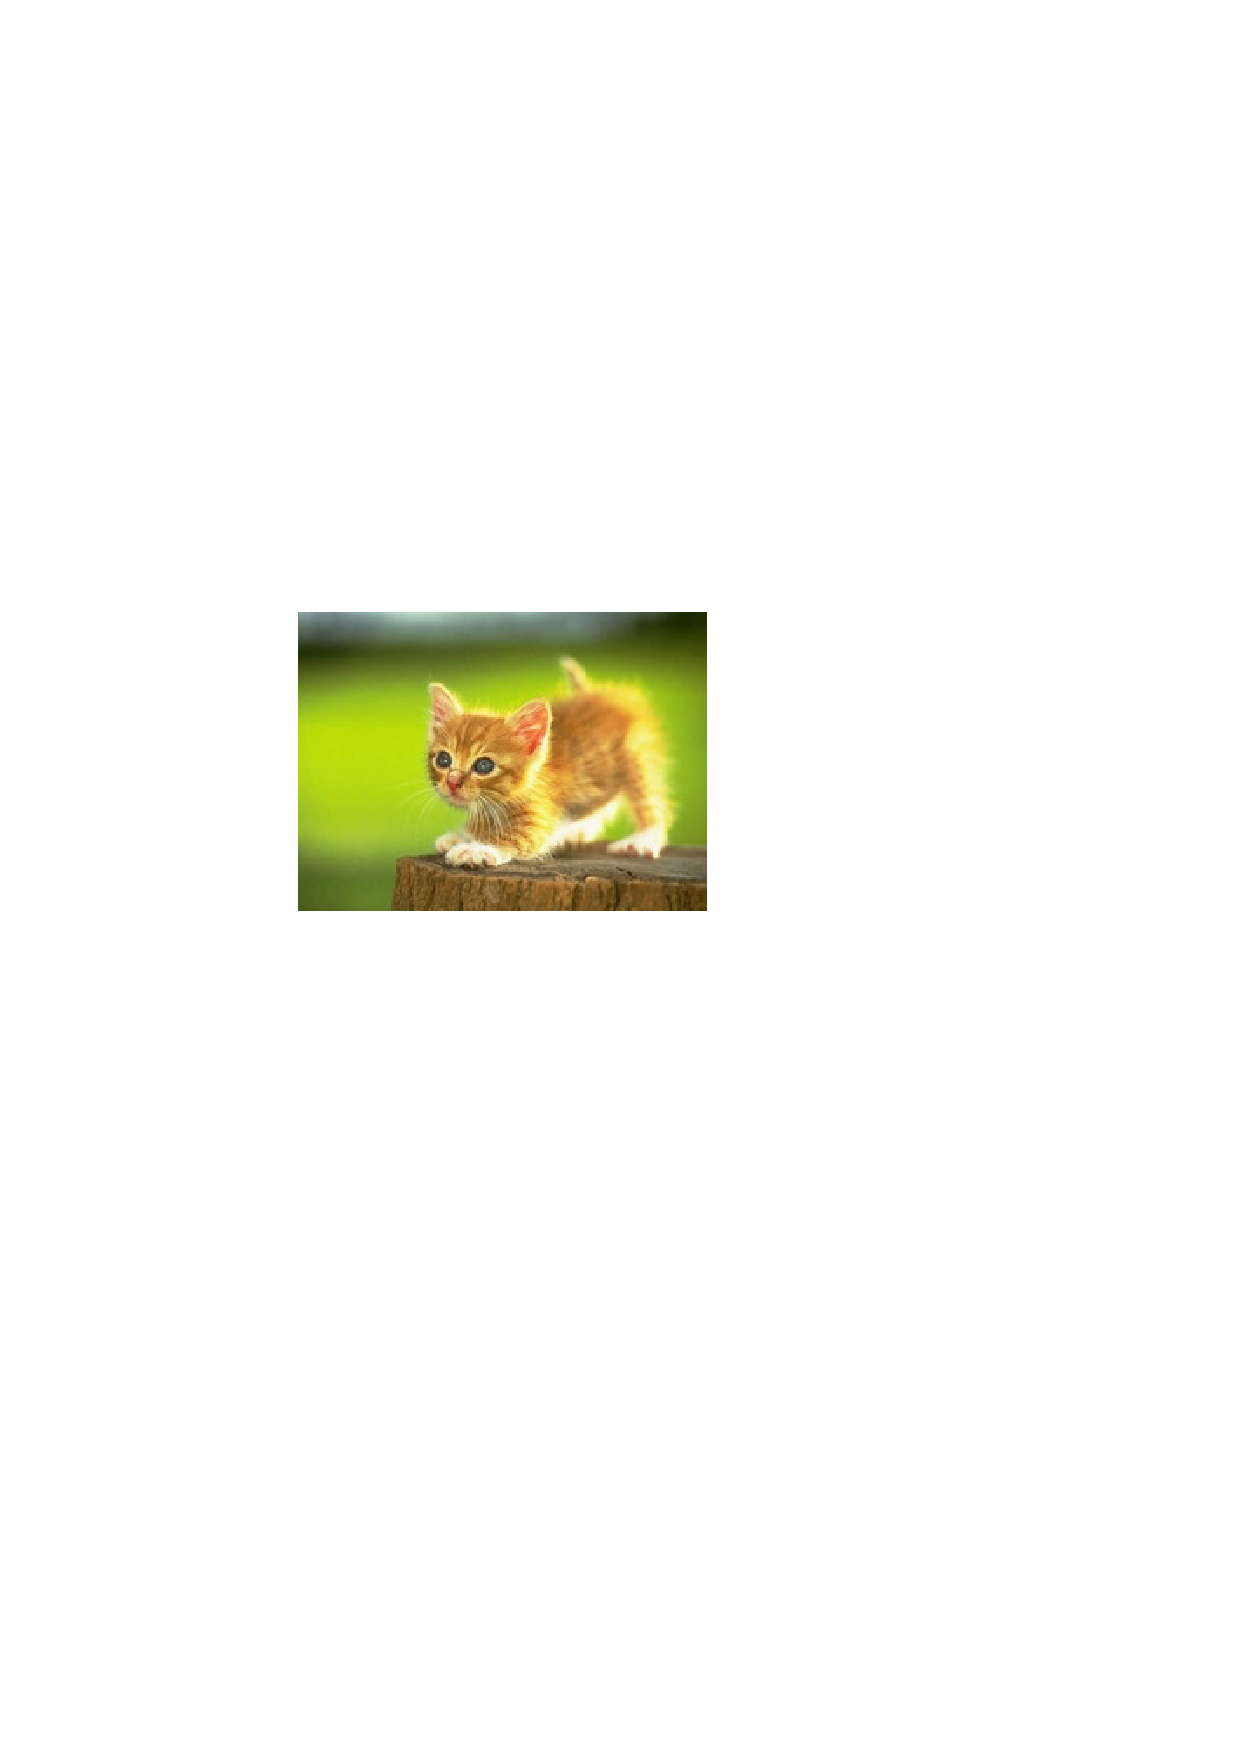
\includegraphics[width=\textwidth]{fig/fig-example.pdf}
  \caption{图片2}\label{fig:2-2}
  \end{subfigure}
\caption{多个图片}\label{fig:2}
\end{figure}

\section{参考文献示例}
这是一篇中文参考文献\cite{TEXGURU99};这是一篇英文参考文献\cite{knuth};同时引用\cite{TEXGURU99,knuth}。

\section[\textbackslash{}autoref 测试]{\texttt{\textbackslash{}autoref} 测试}

\begin{description}
  \item[公式] \autoref{eq:1}
  \item[脚注] \autoref{footnote:1}
  \item[项] \autoref{item:1},\autoref{item:2},\autoref{item:3}
  \item[图] \autoref{fig:1}
  \item[表] \autoref{tab:1}
  \item[附录] \autoref{appendix:1}
  \item[章] \autoref{chapter:BaiscEnv}
  \item[小节] \autoref{sec:Q1},\autoref{sec:Q1_1},\autoref{sec:Q2}
  \item[算法] \autoref{alg:1},\autoref{alg_line:1}
  \item[证明环境] \autoref{def:1},\autoref{proposition:1},\autoref{axiom:1},\autoref{lemma:1},\autoref{theorem:1},\autoref{proof:1}
\end{description}

\backmatter

\begin{ack}
致谢正文。
\end{ack}

\bibliography{ref-example}

\appendix

\begin{publications}
    \item 论文1
    \item 论文2
\end{publications}

\chapter{这是一个附录}\label{appendix:1}
附录正文。


\end{document}
\endinput
%%
%% End of file `hustreport-zh-example.tex'.
